\documentclass{article}
\usepackage[utf8]{inputenc}
\usepackage{float}
\usepackage{amsmath}
\usepackage{graphicx}
\usepackage{minted}
\usepackage{tabularx} % Required package
\usepackage{appendix}
\usepackage[top=2cm, bottom=3cm, left=2.5cm, right=2.5cm]{geometry}
\usepackage{mathtools}
\usepackage[backend=biberm, style=ieee]{biblatex}
% Please add the following required packages to your document preamble:
\usepackage[table,xcdraw]{xcolor}
% Please add the following required packages to your document preamble:
\usepackage{multirow}
% Beamer presentation requires \usepackage{colortbl} instead of 
\usepackage[table,xcdraw]{xcolor}
\addbibresource{references.bib} 
\DeclarePairedDelimiter\abs{\lvert}{\rvert}


% SUCH A SEXY WEBSITE -> https://www.tablesgenerator.com/latex_tables
\title{
\large CMPE4003 -- CPU and GPU Architectures \\
\LARGE Basic 16-bit CPU Implementation Report}
\author{
    Chihab Chamkhi \\
    21498754 \\
    \and
    Xavier Curr \\
    22199456 \\
    \and
    Vishaal Chopra \\
    \and
    Afeef Ahmed
}
\date{October 2026}

\begin{document}

\maketitle

\section{Introduction}
This report outlined the implementation of a 16-bit CPU, even though it was intended to be based as an extension of this existing 8-bit CPU design  \cite{8bitref}. The resulting design has no resemblance to it.

\section{Design Specifications and Architecture Overview}

\subsection{Memory Structures}
Before ISA is defined the memory is defined here.


\begin{table}[H]
\centering
\begin{tabularx}{\linewidth}{|c|l|l|l|>{\raggedright\arraybackslash}X|}
\hline
\textbf{Data Structure} & \textbf{\begin{tabular}[c]{@{}l@{}}ADDRESS\\ BITS\end{tabular}} & \textbf{SIZE} & \textbf{WIDTH} & \textbf{DESCRIPTION}                                                                                           \\ \hline
\rowcolor[HTML]{D9E1F2} 
\textbf{INSTRUCTIONS}   & 9                                                               & 512           & 16             & Instruction Memory is seperated from memory and addressable through 9 bits, thus only 512 instruction programs \\ \hline
\rowcolor[HTML]{FCE4D6} 
\textbf{REGISTERS}      & 3                                                               & 8             & 16             & Registers hold 8x16 bits of data.                                                                              \\ \hline
\rowcolor[HTML]{FFF2CC} 
\textbf{MEMORY}         & 9                                                               & 512           & 16             & Memory file is seperated from Instruction Memory. We can store up to 512x16 but probably dont need it          \\ \hline
\rowcolor[HTML]{E2EFDA} 
\textbf{SWITCHES}       & 0                                                               & 1             & 10             & Switches input data, holds 10 bits, only 1 addressable.                                                        \\ \hline
\rowcolor[HTML]{D6DCE4} 
\textbf{SSD}            & 0                                                               & 1             & 16             & Seven Segment Display output, holds 16 bits, only 1 addressable                                                \\ \hline
\end{tabularx}
\caption{Data structures used in the CPU}
\label{datas}
\end{table}
%
%
%  
\subsection{Instruction Set Architecture}
In table \ref{tab:instructionset} is the instruction set architecture. Even though there are Mnemonics for the various $OPCODE$, based on whether the format type further subdivides the Instruction into component functions those functions will have their own Mnemonics to be used in the assembly writing process. Examples of assembly code can be seen in \ref{sec:codeexamples}.

\begin{table}[!h]
\centering
\begin{tabularx}{\linewidth}{|llll>{\raggedright\arraybackslash}X|}
\hline
\multicolumn{5}{|c|}{OPCODE MAP}                                                                                                                                                                                                                                                                                                                                              \\ \hline
\rowcolor[HTML]{DDEBF7} 
\multicolumn{1}{|l|}{\cellcolor[HTML]{DDEBF7}\textbf{OPCODE}}             & \multicolumn{1}{l|}{\cellcolor[HTML]{DDEBF7}\textbf{MNEMONIC}}           & \multicolumn{1}{l|}{\cellcolor[HTML]{DDEBF7}\textbf{FORMAT}}          & \multicolumn{1}{l|}{\cellcolor[HTML]{DDEBF7}\textbf{BITS}}             & \textbf{DESCRIPTION}                                                  \\ \hline
\rowcolor[HTML]{DDEBF7} 
\multicolumn{1}{|l|}{\cellcolor[HTML]{DDEBF7}0000}                        & \multicolumn{1}{l|}{\cellcolor[HTML]{DDEBF7}NOP}                         & \multicolumn{1}{l|}{\cellcolor[HTML]{DDEBF7}-}                        & \multicolumn{1}{l|}{\cellcolor[HTML]{DDEBF7}16}                        & no operation                                                          \\ \hline
\rowcolor[HTML]{FCE4D6} 
\multicolumn{1}{|l|}{\cellcolor[HTML]{FCE4D6}0001}                        & \multicolumn{1}{l|}{\cellcolor[HTML]{FCE4D6}ALU}                         & \multicolumn{1}{l|}{\cellcolor[HTML]{FCE4D6}R}                        & \multicolumn{1}{l|}{\cellcolor[HTML]{FCE4D6}16}                        & Loads ALU to select arithmetic/logic R type operation                 \\ \hline
\rowcolor[HTML]{E2EFDA} 
\multicolumn{1}{|l|}{\cellcolor[HTML]{E2EFDA}0010}                        & \multicolumn{1}{l|}{\cellcolor[HTML]{E2EFDA}ALUI}                        & \multicolumn{1}{l|}{\cellcolor[HTML]{E2EFDA}R-I}                      & \multicolumn{1}{l|}{\cellcolor[HTML]{E2EFDA}32}                        & Loads ALU to select arithmetic/logic I type operation                 \\ \hline
\rowcolor[HTML]{FFF2CC} 
\multicolumn{1}{|l|}{\cellcolor[HTML]{FFF2CC}0011}                        & \multicolumn{1}{l|}{\cellcolor[HTML]{FFF2CC}LW}                          & \multicolumn{1}{l|}{\cellcolor[HTML]{FFF2CC}I}                        & \multicolumn{1}{l|}{\cellcolor[HTML]{FFF2CC}16}                        & Load word from memory into register                                   \\ \hline
\rowcolor[HTML]{FFF2CC} 
\multicolumn{1}{|l|}{\cellcolor[HTML]{FFF2CC}0100}                        & \multicolumn{1}{l|}{\cellcolor[HTML]{FFF2CC}SW}                          & \multicolumn{1}{l|}{\cellcolor[HTML]{FFF2CC}I}                        & \multicolumn{1}{l|}{\cellcolor[HTML]{FFF2CC}16}                        & Store Word from register into memory                                  \\ \hline
\rowcolor[HTML]{BAFEFF} 
\multicolumn{1}{|l|}{\cellcolor[HTML]{BAFEFF}0101}                        & \multicolumn{1}{l|}{\cellcolor[HTML]{BAFEFF}LDI}                         & \multicolumn{1}{l|}{\cellcolor[HTML]{BAFEFF}LI}                       & \multicolumn{1}{l|}{\cellcolor[HTML]{BAFEFF}32}                        & Loads the Immediate number into register. immediate is a 16 bits word \\ \hline
\rowcolor[HTML]{FFFFFF} 
\multicolumn{1}{|l|}{\cellcolor[HTML]{FFFFFF}0110}                        & \multicolumn{1}{l|}{\cellcolor[HTML]{FFFFFF}}                            & \multicolumn{1}{l|}{\cellcolor[HTML]{FFFFFF}}                         & \multicolumn{1}{l|}{\cellcolor[HTML]{FFFFFF}}                          & Unused.                                                                      \\ \hline
\rowcolor[HTML]{D6DCE4} 
\multicolumn{1}{|l|}{\cellcolor[HTML]{D6DCE4}0111}                        & \multicolumn{1}{l|}{\cellcolor[HTML]{D6DCE4}BR}                          & \multicolumn{1}{l|}{\cellcolor[HTML]{D6DCE4}BR}                       & \multicolumn{1}{l|}{\cellcolor[HTML]{D6DCE4}16}                        & Branch - jumps somethere only if a flag condition holds               \\ \hline
\rowcolor[HTML]{F7DCDC} 
\multicolumn{1}{|l|}{\cellcolor[HTML]{F7DCDC}1000}                        & \multicolumn{1}{l|}{\cellcolor[HTML]{F7DCDC}JMP}                         & \multicolumn{1}{l|}{\cellcolor[HTML]{F7DCDC}J}                        & \multicolumn{1}{l|}{\cellcolor[HTML]{F7DCDC}16}                        & Jump - unconditional jump                                             \\ \hline
\rowcolor[HTML]{F7DCDC} 
\multicolumn{1}{|l|}{\cellcolor[HTML]{F7DCDC}1001}                        & \multicolumn{1}{l|}{\cellcolor[HTML]{F7DCDC}JAL}                         & \multicolumn{1}{l|}{\cellcolor[HTML]{F7DCDC}J}                        & \multicolumn{1}{l|}{\cellcolor[HTML]{F7DCDC}16}                        & Jump and Link                                                         \\ \hline
\rowcolor[HTML]{FCE4D6} 
\multicolumn{1}{|l|}{\cellcolor[HTML]{FCE4D6}1010}                        & \multicolumn{1}{l|}{\cellcolor[HTML]{FCE4D6}JR}                          & \multicolumn{1}{l|}{\cellcolor[HTML]{FCE4D6}-}                        & \multicolumn{1}{l|}{\cellcolor[HTML]{FCE4D6}16}                        & Jump Register                                                         \\ \hline
\rowcolor[HTML]{FCE4D6} 
\multicolumn{1}{|l|}{\cellcolor[HTML]{FCE4D6}1011}                        & \multicolumn{1}{l|}{\cellcolor[HTML]{FCE4D6}SHIFT}                       & \multicolumn{1}{l|}{\cellcolor[HTML]{FCE4D6}R-S}                      & \multicolumn{1}{l|}{\cellcolor[HTML]{FCE4D6}16}                        & Slides bits in the register left or right                             \\ \hline
\rowcolor[HTML]{FCE4D6} 
\multicolumn{1}{|l|}{\cellcolor[HTML]{FCE4D6}1100}                        & \multicolumn{1}{l|}{\cellcolor[HTML]{FCE4D6}ALU2}                        & \multicolumn{1}{l|}{\cellcolor[HTML]{FCE4D6}R}                        & \multicolumn{1}{l|}{\cellcolor[HTML]{FCE4D6}16}                        & Second set of ALU instructions ()                                     \\ \hline
\rowcolor[HTML]{E2EFDA} 
\multicolumn{1}{|l|}{\cellcolor[HTML]{E2EFDA}1101}                        & \multicolumn{1}{l|}{\cellcolor[HTML]{E2EFDA}ALU2I}                       & \multicolumn{1}{l|}{\cellcolor[HTML]{E2EFDA}R-I}                      & \multicolumn{1}{l|}{\cellcolor[HTML]{E2EFDA}32}                        & Second set of ALU instructions with immediate                         \\ \hline
\rowcolor[HTML]{FCE4D6} 
\multicolumn{1}{|l|}{\cellcolor[HTML]{FCE4D6}1110}                        & \multicolumn{1}{l|}{\cellcolor[HTML]{FCE4D6}IO}                          & \multicolumn{1}{l|}{\cellcolor[HTML]{FCE4D6}R}                        & \multicolumn{1}{l|}{\cellcolor[HTML]{FCE4D6}16}                        & Interface w/ Switches and SSD                                         \\ \hline
\rowcolor[HTML]{FFC7CE} 
\multicolumn{1}{|l|}{\cellcolor[HTML]{FFC7CE}{\color[HTML]{9C0006} 1111}} & \multicolumn{1}{l|}{\cellcolor[HTML]{FFC7CE}{\color[HTML]{9C0006} HALT}} & \multicolumn{1}{l|}{\cellcolor[HTML]{FFC7CE}{\color[HTML]{9C0006} -}} & \multicolumn{1}{l|}{\cellcolor[HTML]{FFC7CE}{\color[HTML]{9C0006} 16}} & {\color[HTML]{9C0006} Ends program}                                   \\ \hline
\end{tabularx}
\caption{Instruction Set Architecture used in CPU design.}
\label{tab:instructionset}
\end{table}

\subsubsection{Instruction Types}

Below defines the instruction types used and their respective formats and bit allocations that are used in the CPU design.

\begin{table}[!h]
\centering
\begin{tabular}{|l|lllll}
\hline
\rowcolor[HTML]{FCE4D6} 
\textbf{R:}                                            & \multicolumn{1}{l|}{\cellcolor[HTML]{FCE4D6}\textbf{{[}15..12{]} op}} & \multicolumn{1}{l|}{\cellcolor[HTML]{FCE4D6}\textbf{{[}11..9{]} rd}}   & \multicolumn{1}{l|}{\cellcolor[HTML]{FCE4D6}\textbf{{[}8..6{]} rs}} & \multicolumn{1}{l|}{\cellcolor[HTML]{FCE4D6}\textbf{{[}5..3{]} rt}}  & \multicolumn{1}{l|}{\cellcolor[HTML]{FCE4D6}\textbf{{[}2..0{]} funct}} \\ \hline
\rowcolor[HTML]{FCE4D6} 
\textbf{R-S: (shift)}                                  & \multicolumn{1}{l|}{\cellcolor[HTML]{FCE4D6}\textbf{{[}15..12{]} op}} & \multicolumn{1}{l|}{\cellcolor[HTML]{FCE4D6}\textbf{{[}11..9{]} rd}}   & \multicolumn{1}{l|}{\cellcolor[HTML]{FCE4D6}\textbf{{[}8..6{]} rs}} & \multicolumn{1}{l|}{\cellcolor[HTML]{FCE4D6}\textbf{{[}5..2{]} amt}} & \multicolumn{1}{l|}{\cellcolor[HTML]{FCE4D6}\textbf{{[}1..0{]} funct}} \\ \hline
\rowcolor[HTML]{FFF2CC} 
\textbf{I:}                                            & \multicolumn{1}{l|}{\cellcolor[HTML]{FFF2CC}\textbf{{[}15..12{]} op}} & \multicolumn{1}{l|}{\cellcolor[HTML]{FFF2CC}\textbf{{[}11..9{]} rd}}   & \multicolumn{3}{l}{\cellcolor[HTML]{FFF2CC}\textbf{{[}8..0{]} addr}}                                                                                                                                                \\ \hline
\rowcolor[HTML]{E2EFDA} 
\cellcolor[HTML]{E2EFDA}                               & \multicolumn{1}{l|}{\cellcolor[HTML]{E2EFDA}\textbf{{[}15..12{]} op}} & \multicolumn{1}{l|}{\cellcolor[HTML]{E2EFDA}\textbf{{[}11..9{]} rd}}   & \multicolumn{1}{l|}{\cellcolor[HTML]{E2EFDA}\textbf{{[}8..6{]} rs}} & \multicolumn{1}{c|}{\cellcolor[HTML]{E2EFDA}\textbf{-}}              & \multicolumn{1}{l|}{\cellcolor[HTML]{E2EFDA}\textbf{{[}2..0{]}funct}}  \\ \cline{2-6} 
\rowcolor[HTML]{E2EFDA} 
\multirow{-2}{*}{\cellcolor[HTML]{E2EFDA}\textbf{R-I}} & \multicolumn{5}{l}{\cellcolor[HTML]{E2EFDA}\textbf{{[}15..0{]} imm16}}                                                                                                                                                                                                                                                                                               \\ \hline
\rowcolor[HTML]{BAFEFF} 
\cellcolor[HTML]{BAFEFF}                               & \multicolumn{1}{l|}{\cellcolor[HTML]{BAFEFF}\textbf{{[}15..12{]} op}} & \multicolumn{1}{l|}{\cellcolor[HTML]{BAFEFF}\textbf{{[}11..9{]} rd}}   & \multicolumn{3}{c}{\cellcolor[HTML]{BAFEFF}\textbf{-}}                                                                                                                                                              \\ \cline{2-6} 
\rowcolor[HTML]{BAFEFF} 
\multirow{-2}{*}{\cellcolor[HTML]{BAFEFF}\textbf{LI:}} & \multicolumn{5}{l}{\cellcolor[HTML]{BAFEFF}\textbf{{[}15..0{]} imm16}}                                                                                                                                                                                                                                                                                               \\ \hline
\rowcolor[HTML]{D6DCE4} 
\textbf{BR:}                                           & \multicolumn{1}{l|}{\cellcolor[HTML]{D6DCE4}\textbf{{[}15..12{]} op}} & \multicolumn{1}{l|}{\cellcolor[HTML]{D6DCE4}\textbf{{[}11..9{]} cond}} & \multicolumn{3}{l}{\cellcolor[HTML]{D6DCE4}\textbf{{[}8..0{]} imm9}}                                                                                                                                                \\ \hline
\rowcolor[HTML]{F7DCDC} 
\textbf{J:}                                            & \multicolumn{1}{l|}{\cellcolor[HTML]{F7DCDC}\textbf{{[}15..12{]} op}} & \multicolumn{1}{c|}{\cellcolor[HTML]{F7DCDC}\textbf{-}}                & \multicolumn{3}{l}{\cellcolor[HTML]{F7DCDC}\textbf{{[}8..0{]} imm9}}                                                                                                                                                \\ \hline
\end{tabular}
\caption{Instruction types and their bit formats used.}
\label{instrt}
\end{table}


\subsection{Functions}

\subsubsection{ALU and ALUI Functions}
There are no difference between ALU and ALUI aside from their instruction length, where ALUI is 32-bit and instead of addressing registers for B (rs2) value it instead uses the last 16-bits. The following Functions in Table \ref{tab:ALUfuncs} are shared between them.

\begin{table}[H]
\centering
\begin{tabular}{|
>{\columncolor[HTML]{F7DCDC}\raggedright\arraybackslash}p{2.2cm} 
>{\columncolor[HTML]{E2EFDA}}l l|}
\hline
\multicolumn{3}{|c|}{\cellcolor[HTML]{E7E6E6}\textbf{ALU and ALUI Functions}}                                                                                                                                     \\ \hline
\multicolumn{1}{|>{\raggedright\arraybackslash}p{2.2cm}|}{\cellcolor[HTML]{DDEBF7}\textbf{funct}} & \multicolumn{1}{l|}{\cellcolor[HTML]{DDEBF7}\textbf{MNEMONIC}} & \cellcolor[HTML]{DDEBF7}\textbf{DESCRIPTION} \\ \hline
\multicolumn{1}{|>{\raggedright\arraybackslash}p{2.2cm}|}{\cellcolor[HTML]{F7DCDC}000}            & \multicolumn{1}{l|}{\cellcolor[HTML]{E2EFDA}ADD}               & rd \textless{}= rs + rt                      \\ \hline
\multicolumn{1}{|>{\raggedright\arraybackslash}p{2.2cm}|}{\cellcolor[HTML]{F7DCDC}001}            & \multicolumn{1}{l|}{\cellcolor[HTML]{E2EFDA}SUB}               & rd \textless{}= rs - rt                      \\ \hline
\multicolumn{1}{|>{\raggedright\arraybackslash}p{2.2cm}|}{\cellcolor[HTML]{F7DCDC}010}            & \multicolumn{1}{l|}{\cellcolor[HTML]{E2EFDA}Increment}         & rd \textless{}= rs + 1                       \\ \hline
\multicolumn{1}{|>{\raggedright\arraybackslash}p{2.2cm}|}{\cellcolor[HTML]{F7DCDC}011}            & \multicolumn{1}{l|}{\cellcolor[HTML]{E2EFDA}Decrement}         & rd \textless{}= rs - 1                       \\ \hline
\multicolumn{1}{|>{\raggedright\arraybackslash}p{2.2cm}|}{\cellcolor[HTML]{F7DCDC}100}            & \multicolumn{1}{l|}{\cellcolor[HTML]{E2EFDA}AND}               & rd \textless{}= rs AND rd                    \\ \hline
\multicolumn{1}{|>{\raggedright\arraybackslash}p{2.2cm}|}{\cellcolor[HTML]{F7DCDC}101}            & \multicolumn{1}{l|}{\cellcolor[HTML]{E2EFDA}OR}                & rd \textless{}= rs OR rt                     \\ \hline
\multicolumn{1}{|>{\raggedright\arraybackslash}p{2.2cm}|}{\cellcolor[HTML]{F7DCDC}110}            & \multicolumn{1}{l|}{\cellcolor[HTML]{E2EFDA}XOR}               & rd \textless{}= rs XOR rt                    \\ \hline
\multicolumn{1}{|>{\raggedright\arraybackslash}p{2.2cm}|}{\cellcolor[HTML]{F7DCDC}111}            & \multicolumn{1}{l|}{\cellcolor[HTML]{E2EFDA}NOT}               & rd \textless{}= NOT rs                       \\ \hline
\end{tabular}
\caption{ALU func codes and respective functions}
\label{tab:ALUfuncs}
\end{table}


\subsubsection{ALU2 and ALU2I Functions}

There are no difference between ALU2 and ALU2I aside from their instruction length, where ALU2I is 32-bit and instead of addressing registers for B (rs2) value it instead uses the last 16-bits. The following Functions in Table \ref{tab:alu2funcs} are shared between them.

\begin{table}[H]
\centering
\begin{tabular}{|
>{\columncolor[HTML]{F7DCDC}\raggedright\arraybackslash}p{2.2cm} 
>{\columncolor[HTML]{E2EFDA}}l l|}
\hline
\multicolumn{3}{|c|}{\cellcolor[HTML]{E7E6E6}\textbf{ALU2 and ALU2I Functions}}                                                                                                                                             \\ \hline
\multicolumn{1}{|>{\raggedright\arraybackslash}p{2.2cm}|}{\cellcolor[HTML]{DDEBF7}\textbf{funct}} & \multicolumn{1}{l|}{\cellcolor[HTML]{DDEBF7}\textbf{MNEMONIC}} & \cellcolor[HTML]{DDEBF7}\textbf{DESCRIPTION} \\ \hline
\multicolumn{1}{|>{\raggedright\arraybackslash}p{2.2cm}|}{\cellcolor[HTML]{F7DCDC}000}            & \multicolumn{1}{l|}{\cellcolor[HTML]{E2EFDA}MIN}               & rd\textless{}=min(rs, rt)                    \\ \hline
\multicolumn{1}{|>{\raggedright\arraybackslash}p{2.2cm}|}{\cellcolor[HTML]{F7DCDC}001}            & \multicolumn{1}{l|}{\cellcolor[HTML]{E2EFDA}MAX}               & rd\textless{}=max(rs,rt)                     \\ \hline
\multicolumn{1}{|>{\raggedright\arraybackslash}p{2.2cm}|}{\cellcolor[HTML]{F7DCDC}010}            & \multicolumn{1}{l|}{\cellcolor[HTML]{E2EFDA}MINU}              & rd\textless{}=min(rs, rt)                    \\ \hline
\multicolumn{1}{|>{\raggedright\arraybackslash}p{2.2cm}|}{\cellcolor[HTML]{F7DCDC}011}            & \multicolumn{1}{l|}{\cellcolor[HTML]{E2EFDA}MAXU}              & rd\textless{}=max(rs,rt)                     \\ \hline
\multicolumn{1}{|>{\raggedright\arraybackslash}p{2.2cm}|}{\cellcolor[HTML]{F7DCDC}100}            & \multicolumn{1}{l|}{\cellcolor[HTML]{E2EFDA}NEG}               & rd \textless{}= -rs                          \\ \hline
\multicolumn{1}{|>{\raggedright\arraybackslash}p{2.2cm}|}{\cellcolor[HTML]{F7DCDC}101}            & \multicolumn{1}{l|}{\cellcolor[HTML]{E2EFDA}NAND}              & rd \textless{}= rs NAND rt                   \\ \hline
\multicolumn{1}{|>{\raggedright\arraybackslash}p{2.2cm}|}{\cellcolor[HTML]{F7DCDC}110}            & \multicolumn{1}{l|}{\cellcolor[HTML]{E2EFDA}XNOR}              & rd \textless{}= rs XNOR rt                   \\ \hline
\multicolumn{1}{|>{\raggedright\arraybackslash}p{2.2cm}|}{\cellcolor[HTML]{F7DCDC}111}            & \multicolumn{1}{l|}{\cellcolor[HTML]{E2EFDA}CMP}               & Null \textless{}= rs - rt                    \\ \hline
\end{tabular}
\caption{Table of the functions for ALU2.}
\label{tab:alu2funcs}
\end{table}

\subsubsection{SHIFT Functions}
In table \ref{tab:shftfuncs} are listed the various functions and bits associated for the Shift unit.

\begin{table}[H]
\centering
\begin{tabular}{|
>{\columncolor[HTML]{F7DCDC}}l 
>{\columncolor[HTML]{E2EFDA}}l ll}
\hline
\multicolumn{4}{|c|}{\cellcolor[HTML]{E7E6E6}\textbf{SHIFT FUNCTIONS}}                                                                                                                                     \\ \hline
\multicolumn{1}{|l|}{\cellcolor[HTML]{DDEBF7}\textbf{funct{[}1..0{]}}} & \multicolumn{1}{l|}{\cellcolor[HTML]{DDEBF7}\textbf{MNEMONIC}} & \multicolumn{2}{c}{\cellcolor[HTML]{DDEBF7}\textbf{Description}} \\ \hline
\multicolumn{1}{|l|}{\cellcolor[HTML]{F7DCDC}00}                       & \multicolumn{1}{l|}{\cellcolor[HTML]{E2EFDA}SLL}               & \multicolumn{2}{l|}{Slide left, fill with zeros}                 \\ \hline
\multicolumn{1}{|l|}{\cellcolor[HTML]{F7DCDC}01}                       & \multicolumn{1}{l|}{\cellcolor[HTML]{E2EFDA}SRL}               & \multicolumn{2}{l|}{Slide right, fill with zeros Unsigned}       \\ \hline
\multicolumn{1}{|l|}{\cellcolor[HTML]{F7DCDC}10}                       & \multicolumn{1}{l|}{\cellcolor[HTML]{E2EFDA}SRA}               & \multicolumn{2}{l|}{Slide right arithmetic - signed}             \\ \hline
\multicolumn{1}{|l|}{\cellcolor[HTML]{F7DCDC}11}                       & \multicolumn{1}{l|}{\cellcolor[HTML]{E2EFDA}ROTL}              & \multicolumn{2}{l|}{Rotate left}                                 \\ \hline
\end{tabular}
\caption{Table of the four shift functions, that take 4-bit amount(0-15)}
\label{tab:shftfuncs}
\end{table}


\subsubsection{BR Functions}

In Table \ref{tab:brfuncs} is listed the various function bits required to branch on certain conditions.

\begin{table}[!h]
\centering
\begin{tabularx}{\linewidth}{|
>{\columncolor[HTML]{F7DCDC}}l 
>{\columncolor[HTML]{E2EFDA}}l >{\raggedright\arraybackslash}Xl|}
\hline
\multicolumn{4}{|c|}{\cellcolor[HTML]{DDEBF7}BRANCH CONDITIONS}                                                                                                                                                                                                         \\ \hline
\multicolumn{1}{|l|}{\cellcolor[HTML]{D6DCE4}\textbf{cond}} & \multicolumn{1}{l|}{\cellcolor[HTML]{D6DCE4}\textbf{MNEMONIC}} & \multicolumn{1}{>{\raggedright\arraybackslash}X|}{\cellcolor[HTML]{D6DCE4}\textbf{Branches if}} & \cellcolor[HTML]{D6DCE4}\textbf{Flags} \\ \hline
\multicolumn{1}{|l|}{\cellcolor[HTML]{F7DCDC}000}           & \multicolumn{1}{l|}{\cellcolor[HTML]{E2EFDA}BEQ}               & \multicolumn{1}{>{\raggedright\arraybackslash}X|}{Equal}                                        & Z = 1                                  \\ \hline
\multicolumn{1}{|l|}{\cellcolor[HTML]{F7DCDC}001}           & \multicolumn{1}{l|}{\cellcolor[HTML]{E2EFDA}BNE}               & \multicolumn{1}{>{\raggedright\arraybackslash}X|}{Not Equal}                                    & Z = 0                                  \\ \hline
\multicolumn{1}{|l|}{\cellcolor[HTML]{F7DCDC}010}           & \multicolumn{1}{l|}{\cellcolor[HTML]{E2EFDA}BLT}               & \multicolumn{1}{>{\raggedright\arraybackslash}X|}{Less Than}                                    & N /= V                                 \\ \hline
\multicolumn{1}{|l|}{\cellcolor[HTML]{F7DCDC}011}           & \multicolumn{1}{l|}{\cellcolor[HTML]{E2EFDA}BGE}               & \multicolumn{1}{>{\raggedright\arraybackslash}X|}{Greater or Equal}                             & N = V                                  \\ \hline
\multicolumn{1}{|l|}{\cellcolor[HTML]{F7DCDC}100}           & \multicolumn{1}{l|}{\cellcolor[HTML]{E2EFDA}BLE}               & \multicolumn{1}{>{\raggedright\arraybackslash}X|}{Less or Equal}                                & Z = 1 || N /= V                        \\ \hline
\multicolumn{1}{|l|}{\cellcolor[HTML]{F7DCDC}101}           & \multicolumn{1}{l|}{\cellcolor[HTML]{E2EFDA}BGT}               & \multicolumn{1}{>{\raggedright\arraybackslash}X|}{Greater Than}                                 & Z = 0 || N = V                         \\ \hline
\multicolumn{1}{|l|}{\cellcolor[HTML]{F7DCDC}110}           & \multicolumn{1}{l|}{\cellcolor[HTML]{E2EFDA}BLTU}              & \multicolumn{1}{>{\raggedright\arraybackslash}X|}{Less Than - Unsigned}                         & C = 0                                  \\ \hline
\multicolumn{1}{|l|}{\cellcolor[HTML]{F7DCDC}111}           & \multicolumn{1}{l|}{\cellcolor[HTML]{E2EFDA}BGEU}              & \multicolumn{1}{>{\raggedright\arraybackslash}X|}{Greater or Equal - Unsigned}                  & C = 1                                  \\ \hline
\end{tabularx}
\caption{Funciton Select in branch instrucitons for various conditional jumps.}
\label{tab:brfuncs}
\end{table}
\subsubsection{IO Functions}

In table \ref{tab:iofuncs} the MNEMONICS capable of use for the IO Instruction are shown. 

\begin{table}[H]
\centering
\begin{tabular}{|
>{\columncolor[HTML]{F7DCDC}}l 
>{\columncolor[HTML]{E2EFDA}}l l}
\hline
\multicolumn{3}{|c}{\cellcolor[HTML]{E7E6E6}IO Functions}                                                                                                                                                                                       \\ \hline
\multicolumn{1}{|l|}{\cellcolor[HTML]{D9E1F2}\textbf{funct}}             & \multicolumn{1}{l|}{\cellcolor[HTML]{D9E1F2}\textbf{MNEMONIC}}           & \multicolumn{1}{l|}{\cellcolor[HTML]{D9E1F2}\textbf{DESCRIPTION}}                         \\ \hline
\multicolumn{1}{|l|}{\cellcolor[HTML]{F7DCDC}000}                        & \multicolumn{1}{l|}{\cellcolor[HTML]{E2EFDA}SSD}                         & \multicolumn{1}{l|}{SSD \textless{}= rs}                                                  \\ \hline
\multicolumn{1}{|l|}{\cellcolor[HTML]{F7DCDC}001}                        & \multicolumn{1}{l|}{\cellcolor[HTML]{E2EFDA}SWI}                         & \multicolumn{1}{l|}{rd \textless{}= SW}                                                   \\ \hline
\multicolumn{1}{|l|}{\cellcolor[HTML]{F7DCDC}{\color[HTML]{AEAAAA} 010}} & \multicolumn{1}{l|}{\cellcolor[HTML]{E2EFDA}{\color[HTML]{AEAAAA} SSDI}} & \multicolumn{1}{l|}{{\color[HTML]{AEAAAA} SSD \textless{}= {[}addr{]} * not Implemented}} \\ \hline
\multicolumn{1}{|l|}{\cellcolor[HTML]{F7DCDC}{\color[HTML]{AEAAAA} 011}} & \multicolumn{1}{l|}{\cellcolor[HTML]{E2EFDA}{\color[HTML]{AEAAAA} SWI}}  & \multicolumn{1}{l|}{{\color[HTML]{AEAAAA} {[}addr{]} \textless{}= SW * not Implemented}}  \\ \hline
\end{tabular}
    \caption{Table of IO Functions. There is a lot more room for development and functionality}
    \label{tab:iofuncs}
\end{table}

\section{Component Design and Description}

\subsection{Program Counter (PC)}

The Program Counter used is a combinational unit that updates the output PC based on various control signals from the decode stage. This has the effect that any Program Control/Flow signals that are decoded/executed in the decode stage will immediately effect and update the PC to reduce any bubbles in the pipeline. This allows us to take advantage of this fact and implement the Branch Unit in the decode stage, effectively achieving zero bubble. However a $CMP$ instruction will need to be executed before a branch instruction, so effectively 2 clock pulses are required for a branch but at least this allows us to not have to worry about implementing bubbling. 

Figure \ref{fig:pc} below shows its functional block implementation. A counter is used with the option of $C_{OUT}=C_{IN} +1$, or $C_{OUT}=C_{IN} +2$, this is to alternate between 16 bit instructions or 32-bit instruction since the Instruction memory is Word (16-bit) Addressable rather than Byte addressable -- Otherwise we would have it as +2 and +4. This is by default fed into the DFF (N-bit D Flip Flop) which will store the value upon a rising clock, allowing it be used to update again for $C_{IN}$ in the next clock cycle. The output of this counter is forwarded to both the input of the stack and output as the PC (if selected). The stack would store the PC+1 so that it doesn't enter into an infinite loop as the instruction at that address stored would be a JAL-- So JAL then later JR to JAL and so on repeatedly.

The option to ouput the BUS\_IN value is also available, this option is selected when the JAL and JMP are high where we need the ouptut to be the bus value, so this fed into the output and the input for DFF to be capable of being incremented.

\begin{figure}[H]
    \centering
    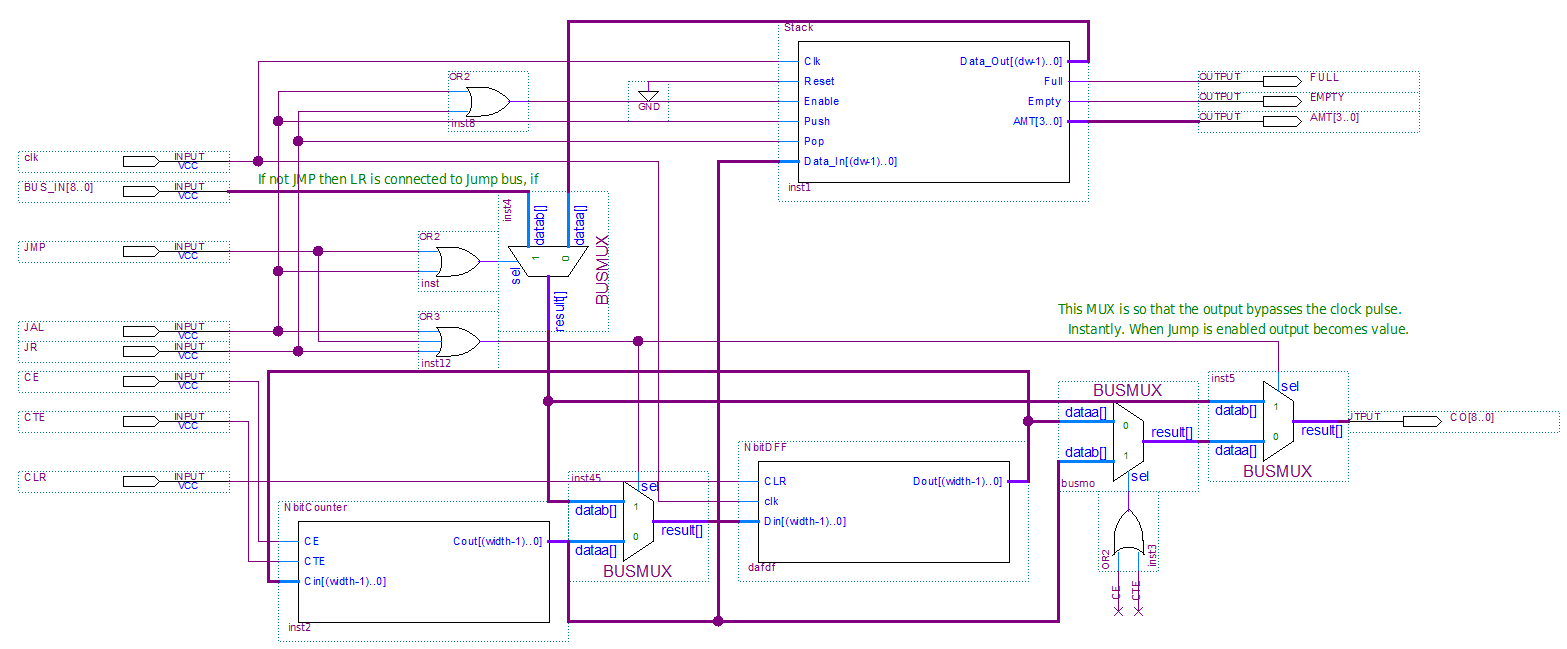
\includegraphics[width=1.1\linewidth]{Components/Program Counter.png}
    \caption{Block Diagram form of the program counter Implementation.}
    \label{fig:pc}
\end{figure}

\begin{table}[H]
    \centering
    \begin{tabularx}{\linewidth}{|c|X|}
\hline
\textbf{INPUT} & \textbf{DESCRIPTION} \\ \hline
clk & Just the clock pulse used in the pipeline stages. This is used to for adding to the stack and setting the N bit DFlip Flop that holds PC of the decode stage.  \\ \hline
BUS\_IN[15..0] & BUS used for setting the PC to a particular value\\ \hline
JMP & The flag to output the BUS\_IN value as the PC. This is for setting the PC to a particular address.\\ \hline
JAL & The flag to ouput the BUS\_IN value as the PC but also add the value it was +1/2 to the Stack, so that it can be jumped back to later. \\ \hline
JR &  This pops the value at the Stack and uses that value as the PC. Used to go back to a particular point in program.\\ \hline
CE & when this signal is on (without CTE on) the count is enabled by +1\\ \hline 
CTE & Count Two Enable. A bit used to increment the $PC_{DEC}$ by 2 instead of 1—This is for 32bit instructions that have an immediate input. When it is set the output is the $PC_{DEC} +2$ \\ \hline
CLR & This is used to clear the D flip flop \\ \hline
    \end{tabularx}
    \caption{Description of functionality of the various input signals of Program Counter}
    \label{tab:input_pc}
\end{table}

\begin{table}[H]
    \centering
    \begin{tabular}{|c|p{15cm}|}
\hline
\textbf{OUTPUT} & \textbf{DESCRIPTION} \\ \hline
FULL & A bit signal to inform that Stack is full. \\ \hline
EMPTY & A bit signal that informs that Stack is empty. \\ \hline
EMPTY[3..0] & A Vector signal for the amount of elements stack holds. \\ \hline

    \end{tabular}
    \caption{Descriptions of the various output signals of Program Counter}
    \label{tab:output_pc}
\end{table}

\subsection{Memory (ROM and RAM)}

The implementation of Memory in this Basic CPU uses two separate Hardware descriptions for Instruction Memory and Random Access Storage Memory. This decision was made to reduce complexity of implementation. Hence this CPU can be said to be of Harvard Architecture. However modern CPU's already separate their instruction memory and storage memory by the time it gets to the CPU, for implementing this we need to partition a RAM which holds both Instruction memory and Data. 

\subsubsection{Instruction Memory (ROM)}

For Instruction Memory define a Read Only Memory (ROM) hardware architecture for its implementation so changes to the program cannot be made on run time. In Figure \ref{fig:ROMentity} the ROM entity used is described in VHDL. The ROM is addressable with 9 bits from the input PC. 9-bits gives us up to $2^9=512$ instructions capable of being loaded at a time. The ROM outputs 2 16-bit Buses one for $PC$ and one for $PC+1$ so that the option to use those later 16-bits for an immediate value is always available. In the CPU implementation the ROM is used similarly to a Pipeline Register holding the output for the decode stage effectively also taking the role as Instruction Register. The output of the ROM updates on every rising clock. Of course in a real CPU if we want to run at higher clock frequencies the ROM cannot take both roles and alternative methods should be considered but for a basic implementation this is fine.     

As can be seen in the definition we in the architecture we have a comment "--START:" under 'ramdef := (' this is where we can load our program to in hexadecimal or binary. 

\begin{figure} [H]
    \centering
    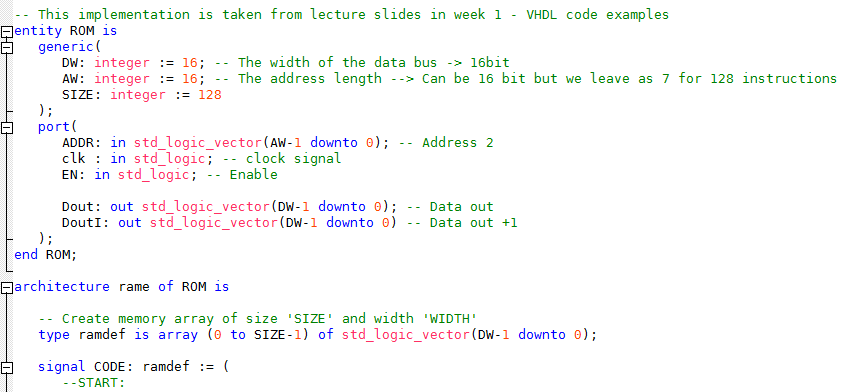
\includegraphics[width=0.9\linewidth]{Components/ROM.png}
    \caption{Rom Implementation for Instruction memory }
    \label{fig:ROMentity}
\end{figure}

\subsubsection{Data Memory (RAM)}

This implementation, shown in figure \ref{ram} is similar to the ROM implementation except it has both a read and write port with 2 address ports--for Data write and Data access--which only has 16-bit input and output buses. This ROM updates its Read port output every rising edge, and writes the input data on every falling edge. It is used similarly to the ROM instruction memory placed in the in-between stages of the pipeline-- In this case it is used in DE/EX intermediary stage, so that data can be accessed as soon as possible, to be forwarded if needed (Otherwise we would need to put a bubble). However for writes this occurs in the useless Write back (WB) stage, of-course in a real CPU writing and reading is not as instant and can take up many clock cycles without a sophisticated caching hierarchal system. This also is word addressable at 9-bits, hence is capable of storing 512 16-bit words.

\begin{figure}[H]
    \centering
    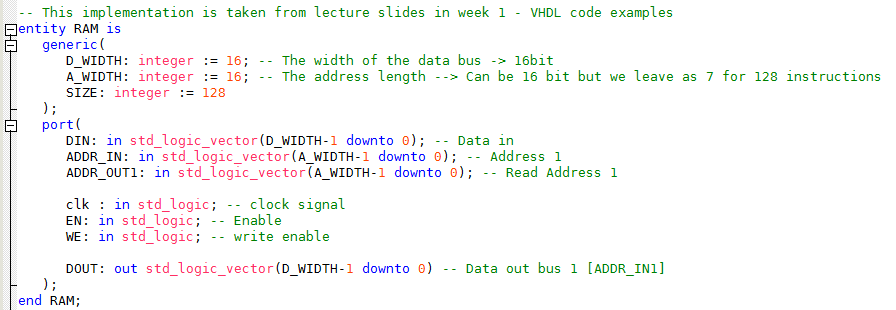
\includegraphics[width=0.9\linewidth]{Components/RAM.png}
    \caption{Random Access Memory for Program Data storage, similar to a heap}
    \label{fig:ram}
\end{figure}


\subsection{Registers}
Registers are implemented with 2 read ports for simultaneous access of A and B for the Execute stage, and one write port to write the results in write back stage. They are 3-bit addressable at the word level (16-bit) for both input and output. Instructions are written on every falling edge. The registers are not read through edge triggered logic, its accessed combination-ally so does not need to wait--Regardless, if edge-triggered access is preferred it can be replaced for the redundant pipeline register that hold the read data. \
Writes can only occur if $ENI$ input is set high, this is because it is connected to shared bus delineation is important.

\begin{figure}[H]
    \centering
    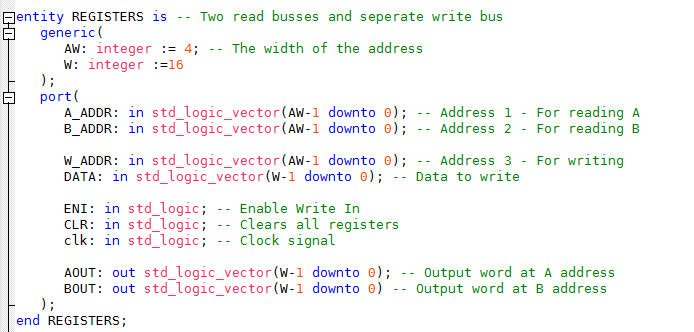
\includegraphics[width=0.9\linewidth]{Components/registers.png}
    \caption{VHDL entity definition of dual-port Registers}
    \label{fig:placeholder}
\end{figure}
\subsection{Control Unit}

The control unit, is the functional component that orchestrates everything for the instruction when it is loaded into the decode stage. From the control units perspective the entire instruction executes at that exact instant combinationally at all stages--It is up to the pipeline Registers to segment the control bits for each stage of the pipeline--therefore for a pipelined CPU the implementation is surprisingly simple and straightforward, refer to the VHDL code below.


\begin{minted}[frame=lines, linenos, fontsize=\footnotesize]{vhdl}
library IEEE;
use IEEE.std_logic_1164.all;
use IEEE.numeric_std.all;
use IEEE.std_logic_unsigned.all;

entity ControlUnit is 
	port(
		OPCODE: in std_logic_vector(3 downto 0); -- The operation that is fetched
		funct: in std_logic_vector(2 downto 0); -- The function of instruction
		
	-- IF/DECODE STAGE
		Halt: out std_logic; -- if Halt set flush=true and CE=false
		Flush: out std_logic;
		
		-- PROGRAM COUNTER
		CE: out std_logic; -- Count Enable increments the count on next rising edge
		CTE: out std_logic;
		JMP: out std_logic;  -- Sets the count to what is on its data bus. J Potential optimization: maybe we could put a register for data in. could save data bus utilization
		JAL: out std_logic; -- Jump and link
		JR: out std_logic; -- Jump to jump register
		BR: out std_logic; -- Branch Instruction
		CLRC: out std_logic; -- count to Clear (straight away) -> no rising edge needed
		
		--Control pipeline from decode stage
		RDIN: out std_logic; -- enable rd as register read into A
		
	 --FW: out std_logic; -- enable forwarding for the instruction *Depricated: Can just use REN bit
	--1. EXECUTE STAGE
		SWO: out std_logic; -- is IO operation
		EXO: out std_logic; -- select A passthrough in Execute
		IMMO: out std_logic; -- Selects Immediate value into bus
		SHFTO: out std_logic; -- Slect shift unit output to out bus
		ALU2: out std_logic; -- Select ALU2 output to execute bus
		MEMO: out std_logic; -- load instruction, memory out
		IMMBO: out std_logic; --select immediate into B of ALU
	--2. WRITEBACK STAGE
	--2.1. INPUT SELECTION
		-- *Depricated
	--2.2. DEVICE SELECTION
		-- REGISTERS
		REN: out std_logic; --Allow write to register
		CLRR: out std_logic;-- Clears the all contents
		-- RAM. 
		MEN: out std_logic; -- Memory Write enable
		-- SSD
		SSEN: out std_logic -- Seven Segment Write Enable
	);
end ControlUnit;

-- Since registers open on rising edge then bits must change on falling edge.
architecture orchestration of ControlUnit is
begin
	process(OPCODE)
	begin
		-- Safe defaults for every output, every time.
		-- Prevents inferred latches and means each branch
		CLRC  <= '0';
		CLRR  <= '0';
		Flush <= '0';
		Halt  <= '0';
		CE    <= '1'; -- Only exception
		CTE   <= '0';
		JMP   <= '0';
		JAL   <= '0';
		JR    <= '0';
		BR    <= '0';
		RDIN  <= '0';
		SWO   <= '0';
		ALU2  <= '0';
		EXO   <= '0';
		IMMBO <= '0';
		SHFTO <= '0';
		IMMO  <= '0';
		MEMO  <= '0';
		MEN   <= '0';
		REN   <= '0';
		SSEN  <= '0';

		-- below only needs to override what's different.
		case OPCODE is
			when "0000" =>  -- NOP
				null;       -- defaults already cover it. Will do nothing in pipeline

			when "0001" =>  -- ALU: rd <= rs, rt
				REN   <= '1'; --Enable Register IN Write 
				
			when "0010" =>  -- ALUI: rd = rs, imm16
				CTE <= '1';
				REN   <= '1'; --Enable Register IN Write 
				IMMBO <= '1'; -- enable immediate operand passthrough

			when "0011" =>  -- LW: rd <= [addr]
				REN   <= '1';
				MEMO 	<= '1'; --select load instruction passthrough to bus
			when "0100" =>  -- SW: [addr] <= rd
				MEN   <= '1'; -- Memory write enable
				EXO 	<= '1'; -- enable A passthrough 
				RDIN 	<= '1';
				
			when "0101" => -- LDI: rd <= imm16
				CTE <= '1';
				REN	<= '1';
				IMMO 	<= '1'; --select imm16 passthrough on bus
			
			when "0110" => --CMP
				null; -- * Depricated
				
			when "0111" => -- BR
				BR 	<= '1';
			when "1000" => -- JMP: IR <= [11..0]
				JMP   <= '1';
			when "1001" =>  -- JAL: push[IR], IR <= [11..0]
				JAL   <= '1';
			when "1010" =>  -- JR: IR <= pop[IR]
				JR   	<= '1';
			when "1011" =>  -- SHIFT: rd<= rs<<amt
				REN 	<= '1';
				SHFTO <= '1';
				
			when "1100" => -- ALU2: 
				if not funct = "111" then -- If not CMP Instruction
					REN  	<= '1'; 
				end if;
				ALU2  <= '1';

			when "1101" => -- ALU2I: 
				CTE <= '1';
				if not funct = "111" then -- If not CMP Instruction
					REN  	<= '1'; 
				end if;
				ALU2  <= '1';
				IMMBO <= '1'; -- enable immediate operand passthrough
				
			when "1110" => -- IO: Instruction register
				if(funct="000") then
					EXO <= '1'; -- Register passthrough to Execute output
					RDIN <='1';
					SSEN <= '1'; --enable Seven Segment Display
				elsif funct="001" then
					SWO <= '1'; -- Enable switch to bus
					REN <= '1'; -- enable register write
				end if;
				
			when "1111" =>
				Halt <= '1'; -- feeds op '1111' into instruction register (endless inescapable feedback)
				CE   <= '0';
			when others =>
				null;-- undefined opcode: hold safe defaults
		end case;
	end process;
end orchestration;
\end{minted}


\subsection{branch Unit}

As previously mentioned, The branch unit is placed in the decode stage to immediately fire control bits to the Program Counter, this effectively enables the Pipeline to never need to stall or have bubbles. The branch unit takes inputs from the flag Latches in the execute stage and uses them to calculate whether the a specific branch condition is met, encoded by another on its inputs. If that condition holds true for those particular set of flags the Branch Unit will enable BR high and jump to the location specified in the instruction by setting the appropriate flags for the Program Counter. This hence depends on previous instruction to set the flags for its decision. Thus to branch 2 instructions must be used.  

Since the branching VHDL is relatively straightforward, the functional block of its use in the decode stage is shown in Figure \ref{fig:branchfunctional}. The CountJump is directly connected to the Program Counter's $JMP$ input.
\begin{figure}[h]
    \centering
    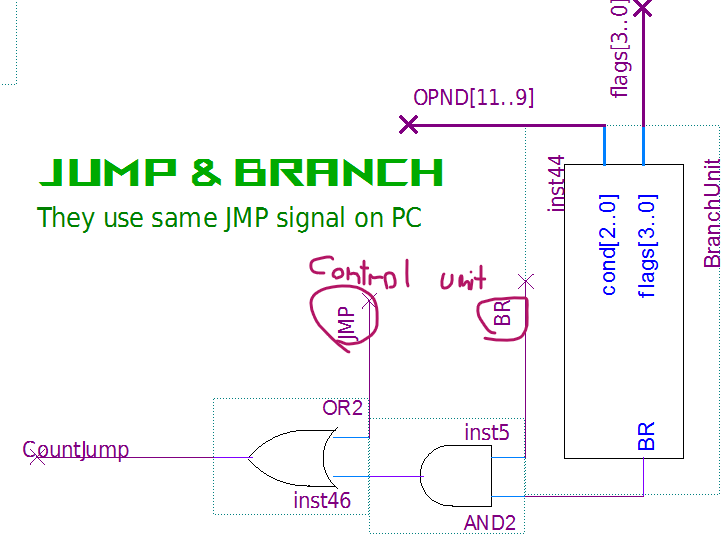
\includegraphics[width=0.4\linewidth]{Components/BranchUnit.png}
    \caption{Jump and branch functional block implementation in CPU.}
    \label{fig:branchfunctional}
\end{figure}


\subsection{Forward Select Unit}

The forward select unit is used to handle data hazards from data that is needed but has not yet been written to the register files due to the nature of the pipeline. To solve this it is required to feedback the resulting values from the proceeding stages if and only if the are required by the instruction in the decode stage--The execute stage value has priority over the Writeback (to be fed forward). 

The functional block diagram of the Forward select Unit is shown in figure \ref{fig:fwdfunctional}. The 'FwdSelectUnit' checks either $A (rs1)$ or $B(rs2)$ addresses against the $C(rd)$ addresses of the write-back and execute stages, if it detects a match it outputs bits that funnel those new values back in-- through the multiplexers shown. Otherwise, pass through the values read from the register file as there should be no conflict with stale values.

\begin{figure}[H]
    \centering
    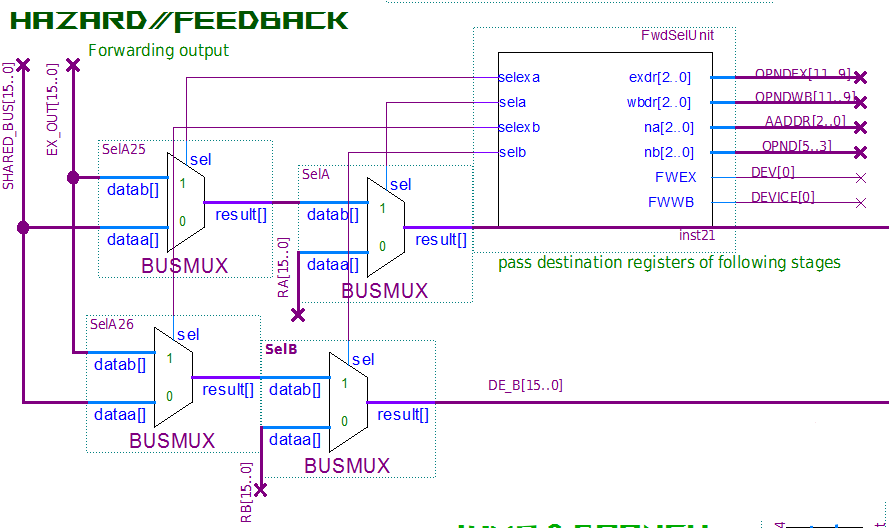
\includegraphics[width=0.7\linewidth]{Components/FwdSelUnit.png}
    \caption{Block Diagram Implementation of Forward select Unit in the CPU.}
    \label{fig:fwdfunctional}
\end{figure}


\subsection{IO (SSD and Switches)}


\section{Top-Level Design and Data Flow }

\subsection{Top-level Pipelined Architecture}

\begin{figure}[H]
    \centering
    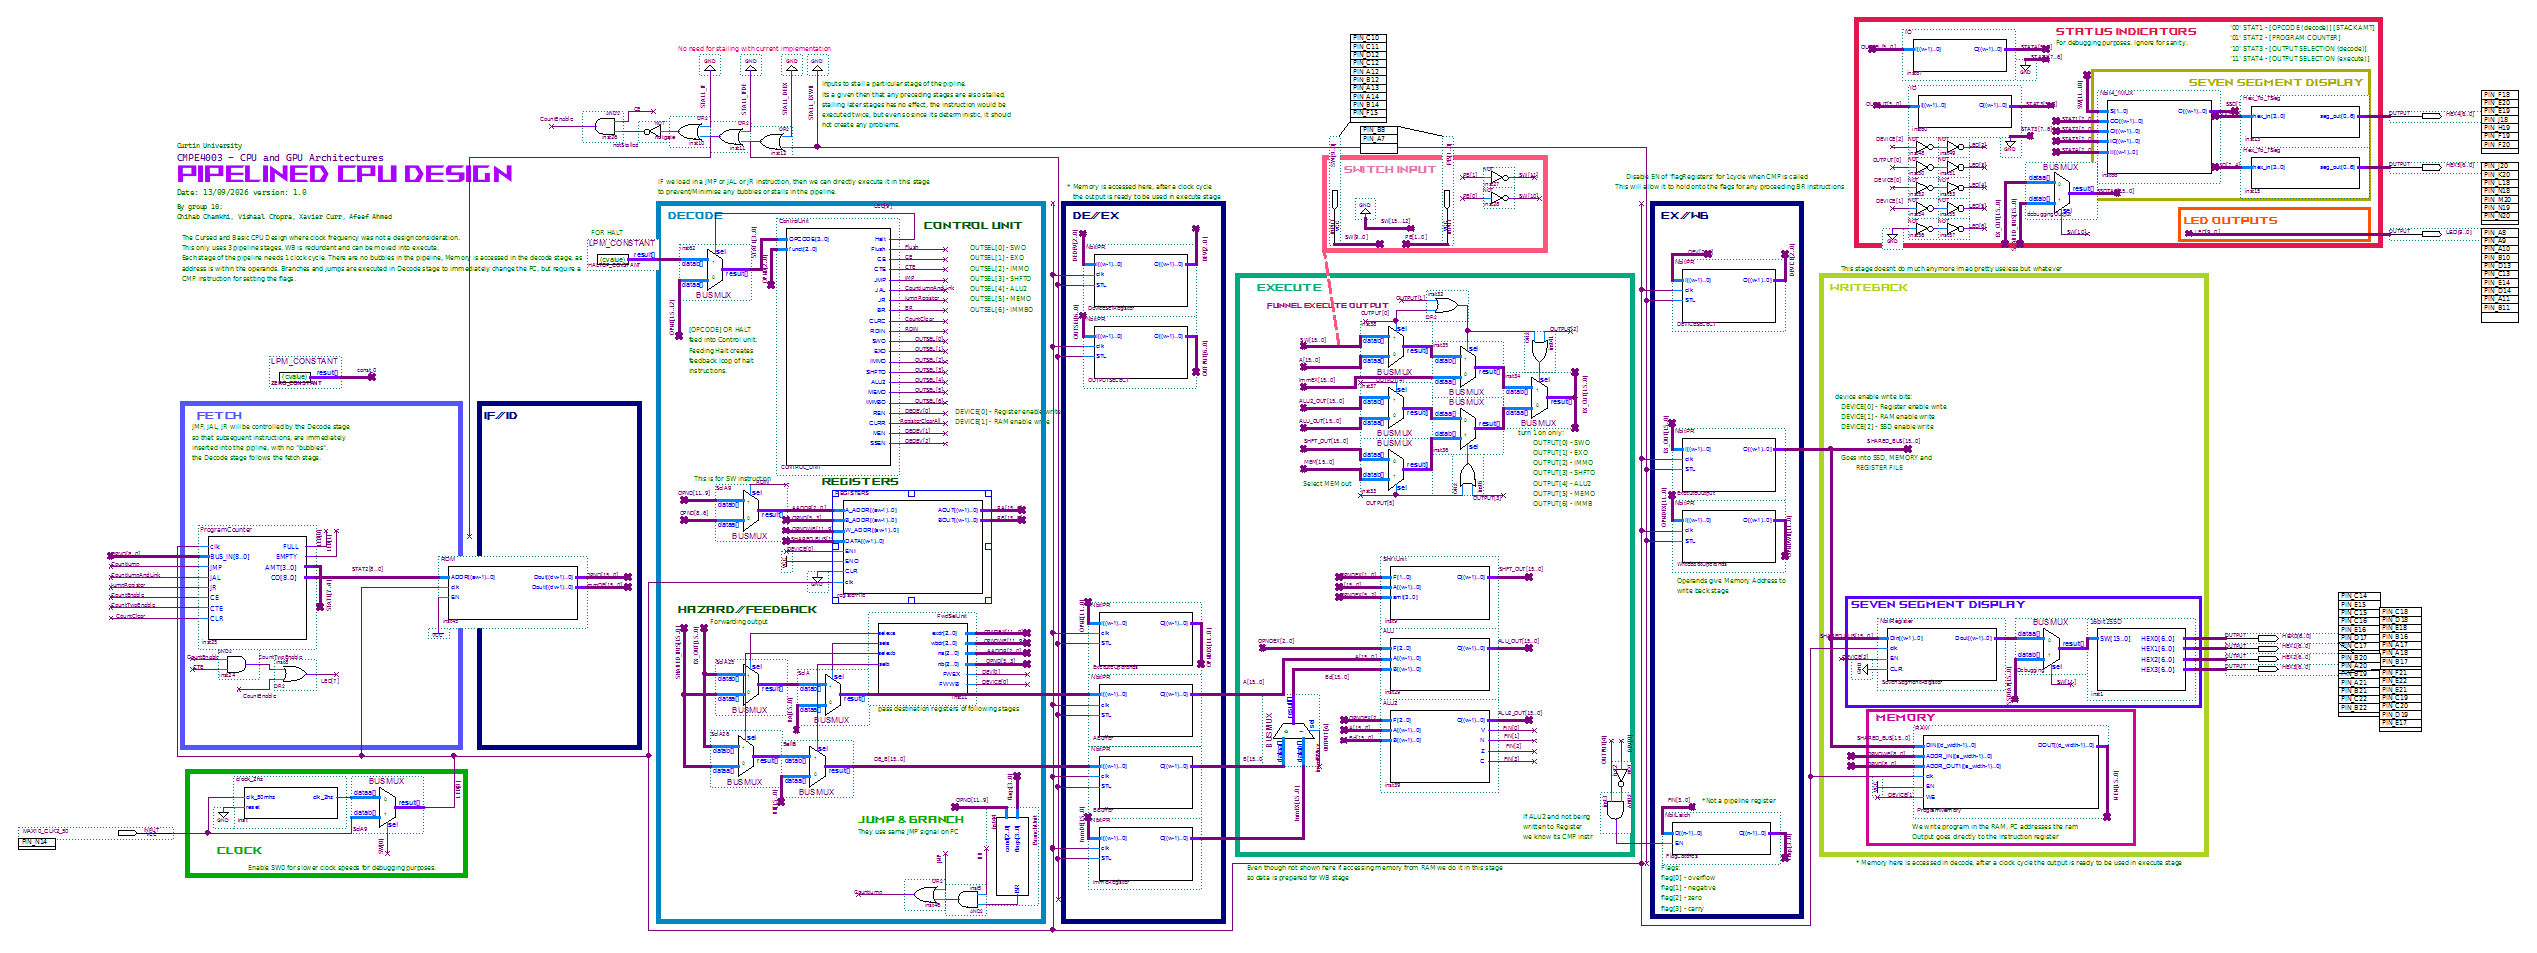
\includegraphics[width=1.1\linewidth]{Components/BasicCPU.png}
    \caption{Top Level view of CPU design. View of Stages and Instruction Flow. }
    \label{fig:placeholder}
\end{figure}

\subsubsection{Fetch Stage}
Fetch pc to memory memory to decode stage

\subsubsection{Decode Stage}
 control unit reads the opcode and asserts signal 
\subsubsection{Execute Stage}

oeprands to the ALU, results generated,

flags updated 

\subsubsection{Writeback Stage}
 result to the register file, ram or Seven Segment Display


Signal and interconnect description – how components are wired 

\subsection{Worked examples walkthrough }

\subsubsection{R-Type ALU Instruction}
(screenshot diagram and write over it) trace it through: 

-Present this as a cycle-by-cycle table alongside annotated diagram that highlights the active path in each stage 

\subsection{J-Type Program Flow instructions}
Second example........... 

\subsection{clock cycles per instruction}

Timing: clock cycles per instruction type in a summary table 

\section{Testing and Verification}
For the simpler components creating testbenches with VHDL with inline assert statements for fast test case checking--the Block Diagram implementations needed to be converted to VHDL for this. These test benches were run on QuestaSim to observe the failure logs, and the waveforms were inspected for debugging. But this Method generally wasn't used extensively for testing as opposed the following. 

Since creating a VHDL test bench for the Basic CPU seemed overwhelmingly annoying, instead a combination of a bunch of Status Indicators connected to LEDs and Seven Segment Displays along with a slow 0.5Hz clock was used to slowly inspect and debug the uploaded CPU. Tables were created for easy access

This method caught a bunch of errors. ..


\section{Discussion}

Overall the CPU Design was successfully implemented and observed to be overall functional. \\
A few changes, we could condense the Instructions Set Architecture even further by combining all the JMP, JAL, JR, into one instruction with a two FUNC bits to select between them... \\

We can also, condense NOP and HALT into one opcode, again using FUNC bits to be able to select between them... \\

This would leave more spaces for other instructions, perhaps ... \\


\section{Conclusion}

This project helped develop skills in VHDL, Block Diagrams, CPU Design, Testing and Verification and the Design considerations in both hardware and Instruction Set Architecture, as well as developing understandings of how Computers work at the basic Level, allowing for exploration in to the more sophisticated and cutting edge designs used in the industry. 

%\bibliographystyle{IEEEtran}
\printbibliography{references}


\appendix
\section{Assembly of Code ran on the CPU}
\subsection{Assembly code for 'echo' program}
\begin{minted}[frame=lines, linenos, fontsize=\footnotesize]{asm}
# =============================================================================
# echo.asm - bring-up test: switches -> display
# =============================================================================
# The smallest possible "is the CPU alive" program. Reads the switches and
# shows the value on the seven-segment display, forever.
#
# Expected: the display always equals the switch value (e.g. all switches
# down -> 0000, SW0 up -> 0001, SW3 and SW0 up -> 0009).
#
# Exercises: SWI, SSD, JMP (backwards).
# =============================================================================

LOOP:
SWI R1
SSD R1
JMP LOOP

\end{minted}

\subsection{Assembly Code for Calc Program}

*Note this is before the addition an Immediate version for ALU2, so some of these instructions may be redundant.

\begin{minted}[frame=lines, linenos, fontsize=\footnotesize]{asm}
# =============================================================================
# calc.asm - interactive switch calculator with peak hold
# =============================================================================
# Reads the switches on every pass, performs one operation and shows the
# result on the seven-segment display, forever. Flip switches while it runs
# and the display follows.
#
# SWITCH LAYOUT (value returned by SWI)
#   SW[3:0]    A     0..15
#   SW[7:4]    B     0..15
#   SW[9:8]    OP    0 = A + B
#                    1 = A - B   (negative shows as 16-bit two's complement,
#                                 e.g. 3 - 4 = FFFF)
#                    2 = A x B   (shift-and-add subroutine)
#                    3 = show PEAK: the largest result seen in OP 0..2
#                        since reset. Hold A = B = 0 with OP = 3 to clear it.
#   SW[15:10]  ignored
#
# THINGS TO TRY (A, B, OP -> display), in this order
#    3,  4, 0 -> 0007        3,  4, 1 -> FFFF        3,  4, 2 -> 000C
#   15, 15, 0 -> 001E       15, 15, 2 -> 00E1       15, 15, 3 -> 00E1 (peak held)
#    0,  0, 3 -> 0000 (peak cleared)
#    9,  2, 0 -> 000B        9,  2, 3 -> 000B (new, lower peak)
#   While OP = 3 the peak stays put however you change A and B, as long as
#   they are not both 0.
#
# REGISTERS
#   R1  raw switch value, later the RESULT
#   R2  temporary                  R3  A (the multiplicand in MULTIPLY)
#   R4  B (the multiplier)         R5  OP
#   R6  constant 0 (never modified after START)
#   R7  link register for JAL/JR (assumed; nothing here keeps data in R7)
#   R0  not used
#
# MEMORY
#   0x1F0  peak value (kept high so it cannot overlap the code)
#
# ASSUMES: CMP sets the flags that BEQ/BNE test and every branch directly
# follows its CMP; JAL saves the return address and JR returns to it;
# SRL shifts right by its amount operand filling with zeros; SLL shifts left;
# MAX is a signed maximum.
#
# Exercises: SWI, SSD, LDI, AND(imm), OR, ADD, SUB, MAX, SLL, SRL, CMP, BEQ,
#            BNE, JMP, JAL, JR, LW, SW.
# =============================================================================

START:
LDI R6 0                    # R6 = 0 for the rest of the run
SW  R6 0x1F0                # peak = 0

MAIN:
SWI R1                      # R1 = raw switches
AND R3 R1 0x0F              # R3 = A = SW[3:0]
SRL R4 R1 4                 # R4 = SW >> 4
AND R4 R4 0x0F              # R4 = B = SW[7:4]
SRL R5 R1 8                 # R5 = SW >> 8
AND R5 R5 0x03              # R5 = OP = SW[9:8]

# ---- choose the operation: OP 0, 1, 2, else 3 ----
CMP R5 R6
BEQ DO_ADD
LDI R2 1
CMP R5 R2
BEQ DO_SUB
LDI R2 2
CMP R5 R2
BEQ DO_MUL
JMP DO_PEAK

DO_ADD:
ADD R1 R3 R4                # result = A + B
JMP UPDATE

DO_SUB:
SUB R1 R3 R4                # result = A - B
JMP UPDATE

DO_MUL:
JAL MULTIPLY                # result = A x B
JMP UPDATE

DO_PEAK:                    # OP 3: show (or clear) the peak
OR  R2 R3 R4                # R2 = A | B
CMP R2 R6
BNE PEAK_SHOW               # some value switch is up -> just show the peak
SW  R6 0x1F0                # A = B = 0 -> clear the peak
PEAK_SHOW:
LW  R1 0x1F0
JMP SHOW

UPDATE:                     # remember the biggest result so far
LW  R2 0x1F0
MAX R2 R2 R1
SW  R2 0x1F0

SHOW:
SSD R1
JMP MAIN

# subroutine: R1 = R3 x R4 by shift-and-add; clobbers R2, R3, R4
MULTIPLY:
LDI R1 0                    # accumulator
MUL_LOOP:
CMP R4 R6                   # multiplier used up?
BEQ MUL_DONE
AND R2 R4 1                 # lowest bit of the multiplier
CMP R2 R6
BEQ MUL_SKIP                # bit clear -> nothing to add
ADD R1 R1 R3                # accumulator += multiplicand
MUL_SKIP:
SLL R3 R3 1                 # multiplicand *= 2
SRL R4 R4 1                 # multiplier /= 2
JMP MUL_LOOP
MUL_DONE:
JR


\end{minted}

\section{Testing. Decoding Tables}

\begin{table}[H]
\centering
\begin{tabular}{|ll|}
\hline
\rowcolor[HTML]{FFCE93} 
\multicolumn{2}{|l|}{\cellcolor[HTML]{FFCE93}\textbf{EXECUTE OUPUT CONTROL DEFINITIONS}}                                                                 \\ \hline
\rowcolor[HTML]{FFFFC7} 
\multicolumn{1}{|l|}{\cellcolor[HTML]{FFFFC7}\textbf{OUTPUT CODE}} & \textbf{Description}                                                                \\ \hline
\multicolumn{1}{|l|}{01}                                           & IO is on either Switch to execute output or Seven Segment Register In (Check LEDR2) \\ \hline
\multicolumn{1}{|l|}{02}                                           & A Register (rs1) pass through to execute ouptut                                     \\ \hline
\multicolumn{1}{|l|}{04}                                           & Immediate to execute output                                                         \\ \hline
\multicolumn{1}{|l|}{08}                                           & Shift Unit to execute output                                                        \\ \hline
\multicolumn{1}{|l|}{10}                                           & ALU2 Unit to execute output                                                         \\ \hline
\multicolumn{1}{|l|}{20}                                           & Ram Memory to execute output                                                        \\ \hline
\multicolumn{1}{|l|}{40}                                           &                                                                                     \\ \hline
\end{tabular}
\caption{Code used to decode the funnel output in execute stage of the pipeline.}
\label{tab:decode1}
\end{table}

\begin{table}[H]
    \centering
    \begin{tabular}{{|c|p{15cm}|}}
\hline
\textbf{LED ID} & \textbf{Signal Description} \\ \hline
0 & Stack is Full \\ \hline
1 & Stack is Empty \\ \hline
2 & Seven Segment Display Register is on Write Enable \\ \hline
3 & SWO is enabled (Switch input to execute output) \\ \hline
4 & Register is being written to \\ \hline
5 & \\ \hline
6 & \\ \hline
7 & Count is enabled (Either by +2 or +1) \\ \hline
8 & Clock Signal \\ \hline
9 & If on Program is halted. \\ \hline


    \end{tabular}
    \caption{Table used to decode CPU functionality with LEDs.}
    \label{tab:decode2}
\end{table}

\begin{table}[H]
    \centering
    \begin{tabular}{|c|p{15cm}|}
\hline
\textbf{Push Button} & \textbf{Description} \\ \hline
00 & Displays the OPCODE in decode and Amt of Items in the stack \\ \hline
01 & Displays the Program Counter value (Address for ROM) \\ \hline
10 & Displays the EXECUTE output CODE (Refer to table above \ref{tab:decode1}) \\ \hline
11 & \\ \hline
    \end{tabular}
    \caption{Table for selecting output (with push button switches) onto seven segment display 5 and 6. }
    \label{tab:decode3}
\end{table}


\section{Assembler}
\subsection{Code Examples}
\label{sec:codeexamples}


\end{document}
